\documentclass{article}


\usepackage{arxiv}

\usepackage{placeins}
\usepackage[utf8]{inputenc} % allow utf-8 input
\usepackage[T1]{fontenc}    % use 8-bit T1 fonts
\usepackage{hyperref}       % hyperlinks
\usepackage{url}            % simple URL typesetting
\usepackage{booktabs}       % professional-quality tables
\usepackage{amsfonts}       % blackboard math symbols
\usepackage{nicefrac}       % compact symbols for 1/2, etc.
\usepackage{microtype}      % microtypography

\usepackage{graphicx}	% to insert graphs
\usepackage{caption}	% to customize caption style
\usepackage{float}
\usepackage{subfigure}

\usepackage{amsmath}

\title{COMP0037 ASSIGNMENT 3}


\author{
 Group: \texttt{Group L}\\\\
 \textbf{Members:} \texttt{Yun Fang, Yusi Zhou}
}

%\date{}

\begin{document}

\maketitle

\captionsetup[figure]{labelformat={default},labelsep=period,name={Fig.}}

% -------------------------------------------------------------------------------------------
\section{Decision Re-Plan Policy}

Suppose B1 is the cell where the robot first detects the obstacle $O_{B}$. 

Suppose C1 is a cell on the aisle C at the same horizontal level as B1, as illustrated in the Figure 1-c on the assignment sheet. 

Let $T_{W}$ be the time the robot has to wait after the obstacle has been discovered.

Let c be the cost function associated with the path, where $c(L(\pi)) = \mathbb{E}(L(\pi)) $. \\

Note that:

$L_{XY}$ is the shortest path length between two cells X and Y, 

$T$ is the number of timesteps the obstacle remains in front of the robot where $ T = 0.5/ \lambda_{B} + \widetilde{T}$ with $\mathbb{E}(t) = 1/\lambda_{B}$ and $\mathbb{E}(\tilde{t}) = 0.5/ \lambda_{B}$ , 

$L_{W}$ is the cost of waiting a timestep.

% ------------------
\subsection{}

Let $\pi_{1}$ be the policy that the robot waits for the obstacle $O_{B}$ to clear.

Let $\pi_{2}$ be the policy that the robot plans a new path down aisle C.

Then,
\begin{align*}
c(L(\pi_{1})) &= c(L_{IB_{1}} + T_{W} \cdot L_{W} + L_{B_{1}B} + L_{BC} + L_{CG}) \\
c(L(\pi_{2})) &= c(L_{IB_{1}} +  L_{B_{1}C_{1}} + L_{C_{1}C} + L_{CG}) \\
\end{align*}

When, on average, the waiting policy is better than the other one: 
\begin{align*}
c(L(\pi_{1})) &\leq c(L(\pi_{2}))  \\
\mathbb{E}(L(\pi_{1})) &\leq \mathbb{E}(L(\pi_{2}))  \\
\mathbb{E}(L_{IB_{1}} + T_{W} \cdot L_{W} + L_{B_{1}B} + L_{BC} + L_{CG}) &\leq \mathbb{E}(L_{IB_{1}} +  L_{B_{1}C_{1}} + L_{C_{1}C} + L_{CG})  \\
\mathbb{E}(T_{W} \cdot L_{W} + L_{B_{1}B} + L_{BC}) &\leq \mathbb{E}(L_{B_{1}C_{1}} + L_{C_{1}C})  \\
\end{align*}

Because $L_{XY}$ is constant, $L_{W}$ is constant, and $L_{B_{1}B} = L_{C_{1}C}$:
\begin{align*}
\mathbb{E}(T_{W}) \cdot L_{W} + L_{BC} &\leq L_{B_{1}C_{1}}  \\
\mathbb{E}(T_{W}) \cdot L_{W} &\leq L_{B_{1}C_{1}} -  L_{BC}   \\
\mathbb{E}(T_{W}) &\leq \frac{L_{B_{1}C_{1}} -  L_{BC}}{L_{W} }   \\
\end{align*}

In this case, $T_{W} = 1 \cdot T = T$ , so:
\begin{align*}
\mathbb{E}(T) &\leq \frac{L_{B_{1}C_{1}} -  L_{BC}}{L_{W} }   \\
\frac{1}{\lambda_{B}} &\leq \frac{L_{B_{1}C_{1}} -  L_{BC}}{L_{W} }  \\
\lambda_{B} &\geq \frac{L_{W}} {L_{B_{1}C_{1}} -  L_{BC}} \\
\end{align*}

Therefore, the smallest value of $\lambda_{B}$ which guarantees on average that waiting is the better strategy is $\frac{L_{W}} {L_{B_{1}C_{1}} -  L_{BC}}$ and $\lambda_{B} \ne 0$ .

% ------------------
\subsection{}

Let $\pi_{0}$ be the policy that the robot drives directly down aisle B.

Let $\pi_{1}$ be the policy that the robot drives down aisle B, encounters an obstacle and waits.

Let $\pi_{2}$ be the policy that the robot drives down aisle B, encounters an obstacle, drives down aisle C.

Let $\pi_{3}$ be the policy that the robot drives directly down aisle C.

As $L(\pi_{0}) = L(\pi_{3})$ and thus $c(L(\pi_{0}) )= c(L(\pi_{3}))$, we will not discuss $\pi_{0}$ here. \\

Then,
\begin{align*}
c(L(\pi_{1})) &= c(L_{IB_{1}} + T_{W} \cdot L_{W} + L_{B_{1}B} + L_{BC} + L_{CG})\\
c(L(\pi_{2})) &= c(L_{IB_{1}} +  L_{B_{1}C_{1}} + L_{C_{1}C} + L_{CG}) \\
c(L(\pi_{3})) &= c(L_{IC_{1}} +  L_{C_{1}C} + L_{CG}) \\
\end{align*}

If the robot decides to drive directly down aisle C, then:
\begin{align}
c(L(\pi_{3})) &\leq c(L(\pi_{1})) \\
c(L(\pi_{3})) &\leq c(L(\pi_{2}))
\end{align}

by (1) - (2):
\begin{align*}
0 &\leq c(L(\pi_{1})) - c(L(\pi_{2})) \\
0 &\leq \mathbb{E}(L_{IB_{1}} + T_{W} \cdot L_{W} + L_{B_{1}B} + L_{BC} + L_{CG}) - \mathbb{E}(L_{IB_{1}} +  L_{B_{1}C_{1}} + L_{C_{1}C} + L_{CG}) \\
0 &\leq \mathbb{E} (T_{W}) \cdot L_{W} + L_{BC} - L_{B_{1}C_{1}} \\
\mathbb{E} (T_{W}) & \geq \frac{L_{B_{1}C_{1}} - L_{BC}} {L_{W}} \\
\mathbb{E} (T) & \geq \frac{L_{B_{1}C_{1}} - L_{BC}} {L_{W}} \\
\frac{1}{\lambda_{B}} & \geq \frac{L_{B_{1}C_{1}} - L_{BC}} {L_{W}} \\
\lambda_{B} & \leq \frac{L_{W}} {L_{B_{1}C_{1}} - L_{BC}} \\
\end{align*}

Therefore, the maximum value of $\lambda_{B}$ at which the robot will decide to drive directly down C and not attempt to drive down aisle B is $\frac{L_{W}} {L_{B_{1}C_{1}} - L_{BC}}$ and $\lambda_{B} \ne 0$ .

% ------------------
\subsection{}
In this case, $T_{W} = p_{B} \cdot T + (1 - p_{B}) \cdot 0 = p_{B} \cdot T$.

As $p_{B}$ is constant, $\mathbb{E}(T_{W}) = p_{B} \cdot \mathbb{E}(T) =  p_{B} / \lambda_{B}$. \\


Let $\pi_{1}$ be the policy that the robot drives down aisle B, encounters an obstacle and waits.

Let $\pi_{2}$ be the policy that the robot drives down aisle B, encounters an obstacle, drives down aisle C.

Let $\pi_{3}$ be the policy that the robot drives directly down aisle C.

Since in this situation the robot attempts to drive down aisle B first:
\begin{align}
c(L(\pi_{3})) &\geq c(L(\pi_{1})) \\
c(L(\pi_{3})) &\geq c(L(\pi_{2}))
\end{align}

Similarly as in the section 1.2, we can obtain that: 
\[
\mathbb{E} (T_{W}) \leq \frac{L_{B_{1}C_{1}} - L_{BC}} {L_{W}}
\]

As $\mathbb{E}(T_{W}) = p_{B} / \lambda_{B}$, $\lambda_{B}$ is a fixed value and $ \lambda_{B} \ne 0$,
\begin{align*}
p_{B} / \lambda_{B} &\leq \frac{L_{B_{1}C_{1}} - L_{BC}} {L_{W}} \\
p_{B}  &\leq \frac{\lambda_{B}(L_{B_{1}C_{1}} - L_{BC})} {L_{W}}
\end{align*}

Therefore, when $p_{B}$ is below $\frac{\lambda_{B}(L_{B_{1}C_{1}} - L_{BC})} {L_{W}}$, the robot will attempt to drive aisle B first.

% ------------------
\subsection{}

Let $\pi_{1}$ be the policy that the robot drives down aisle B and waits.

Let $\pi_{2}$ be the policy that the robot drives down aisle B, encounters an obstacle $O_{B}$, and drives down aisle C.

Let $\pi_{3}$ be the policy that the robot drives down aisle B, encounters an obstacle $O_{B}$, drives down aisle C, and waits.

Let $\pi_{4}$ be the policy that the robot drives down aisle B, encounters an obstacle $O_{B}$, drives down aisle C, encounters an obstacle $O_{C}$, and drives down aisle D.

Let $\pi_{5}$ be the policy that the robot drives directly down aisle D.

Suppose D1 is a cell on the aisle D at the same horizontal level as B1 and C1.

Then,
\begin{align*}
c(L(\pi_{1})) &= c(L_{IB_{1}} + T_{WB} \cdot L_{W} + L_{B_{1}B} + L_{BC} + L_{CG})\\
c(L(\pi_{2})) &= c(L_{IB_{1}} +  L_{B_{1}C_{1}} + L_{C_{1}C} + L_{CG}) \\
c(L(\pi_{3})) &= c(L_{IB_{1}} +  L_{B_{1}C_{1}} + T_{WC} \cdot L_{W}  + L_{C_{1}C} + L_{CG}) \\
c(L(\pi_{4})) &= c(L_{IB_{1}} +  L_{B_{1}C_{1}} +  L_{C_{1}D_{1}} + L_{D_{1}D} + L_{DG}) \\
c(L(\pi_{5})) &= c(L_{ID_{1}} +  L_{D_{1}D} + L_{DG}) \\
\end{align*}

And,
\begin{align*}
\mathbb{E}(T_{WB}) &=  p_{B} / \lambda_{B} \\
\mathbb{E}(T_{WC}) &=  p_{C} / \lambda_{C}
\end{align*}

We are looking to the path length, so if the robot drives directly down aisle D, it means:
\begin{align}
L(\pi_{5}) &\leq L(\pi_{1}) \\
L(\pi_{5}) &\leq L(\pi_{2}) \\
L(\pi_{5}) &\leq L(\pi_{3}) \\
L(\pi_{5}) &\leq L(\pi_{4}) \\
\end{align}

Sum up the four equation, we obtain that:
\begin{align*}
4 L(\pi_{5}) &\leq 4L_{IB_{1}}  + \mathbb{E}(T_{WB}) \cdot L_{W} +  \mathbb{E}(T_{WC}) \cdot L_{W}  
			+ 3 L_{B_{1}C_{1}} + L_{C_{1}D_{1}} + 4 L_{B_{1}B} 
			+ L_{BC} + 3L_{CG} + L_{DG} \\
4 L(\pi_{5}) &\leq 4L_{IB_{1}}  + (p_{B} / \lambda_{B}   +  p_{C} / \lambda_{C}) \cdot L_{W}  
			+ 3 L_{B_{1}C_{1}} + L_{C_{1}D_{1}} + 4 L_{B_{1}B} 
			+ L_{BC} + 3L_{CG} + L_{DG} \\
4 L(\pi_{5}) &\leq 4L_{IB_{1}}  + (p_{B} / \lambda_{B}   +  p_{C} / \lambda_{C}) \cdot L_{W}  
			+ 4 L_{B_{1}C_{1}} + 4 L_{B_{1}B} 
			+ 4L_{CG} \\
L(\pi_{5}) &\leq L_{IB_{1}}  + (p_{B} / \lambda_{B}   +  p_{C} / \lambda_{C}) \cdot 0.25L_{W}  
			+ L_{B_{1}C_{1}} + L_{B_{1}B} 
			+ L_{CG} \\
L(\pi_{5}) &\leq L_{IB_{1}}  + (p_{B} / \lambda_{B}   +  p_{C} / \lambda_{C}) \cdot 0.25L_{W}  
			+ L_{B_{1}C_{1}} + L_{C_{1}C} 
			+ L_{CG} \\
\end{align*}

Let L be the path length of $(L_{IB_{1}}  
			+ L_{B_{1}C_{1}} + L_{C_{1}C} 
			+ L_{CG} )$
			
Therefore, the upper bound on the value of the path length of the path going down aisle is $L+ 0.25L_{W}\cdot(p_{B} / \lambda_{B}   +  p_{C} / \lambda_{C})$.

\pagebreak
% -------------------------------------------------------------------------------------------
\section{Implement System in ROS}

% ------------------
\subsection{}

We first add a function in the class which returns a cell coordinate as the intermediate destination, according to the aisle passed in. Then in the \textit{planPathToGoalViaAisle()}, we call this function to get the intermediate cell coordinate and search a path from the given start cell to the intermediate cell. If there was a path then we extract and store this path and then search the second path which is from the intermediate cell to the given goal cell. If the second path existed, we extract it and link it to the first one using the provided function \textit{addToEnd()}. At the end of this function we call the \textit{searchGridDraw} to show the first path so that the two paths can be seen simultaneously.


The result is shown in Fig. \ref{performance2.1}. The start point is marked purple, the intermediate cell is marked green, and the goal is marked blue.

\begin{figure}[H]
\centering  
\subfigure[Via Aisle A]{
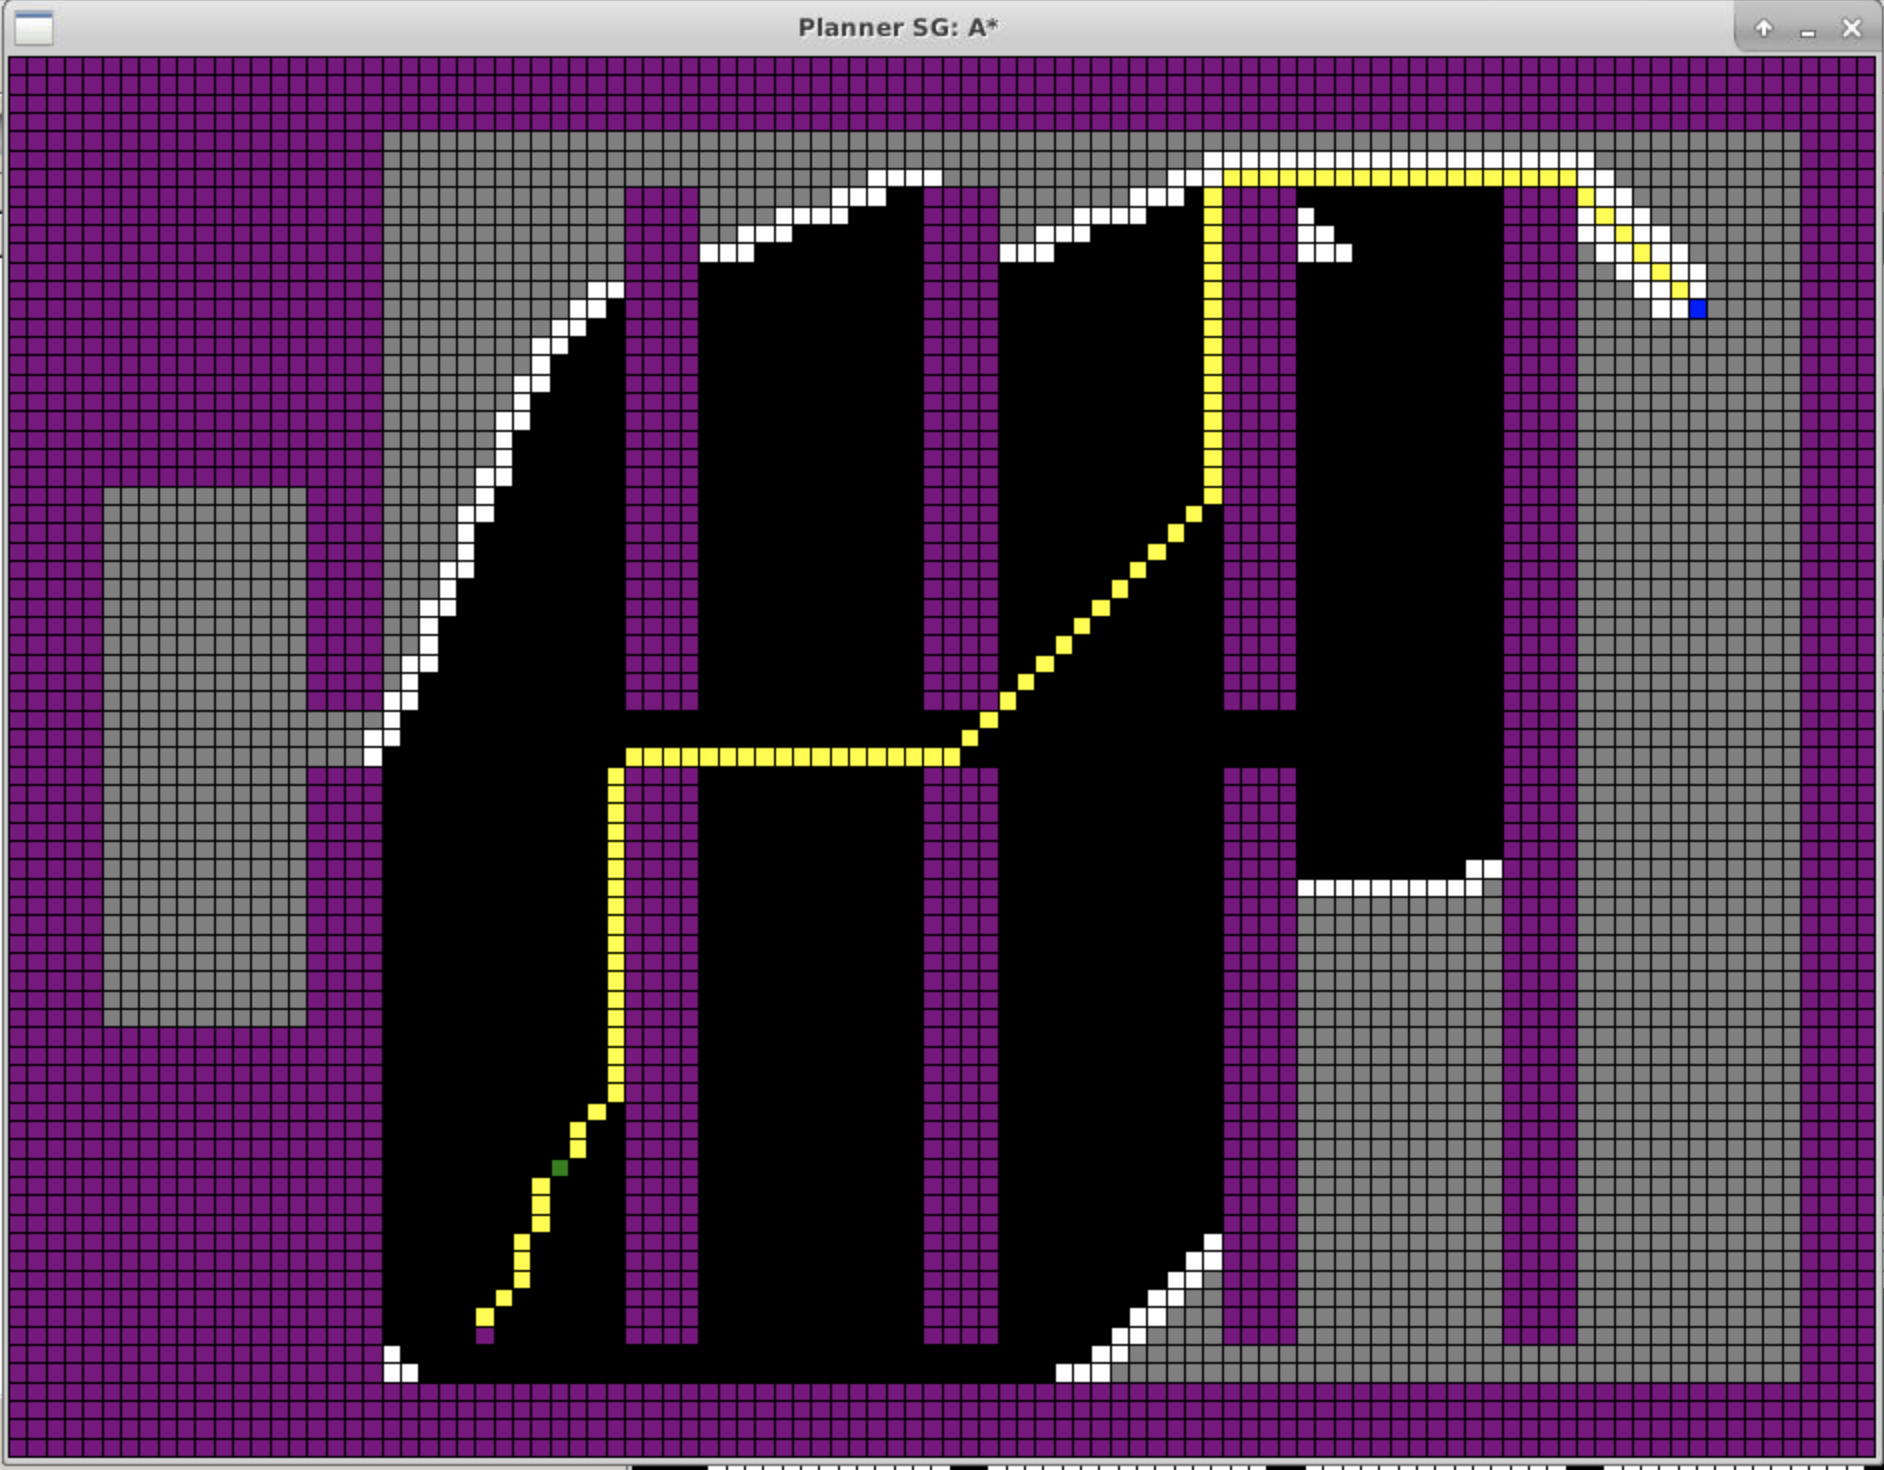
\includegraphics[width=0.32\textwidth]{graphs/part2/2-1/A.png}}
\subfigure[Via Aisle B]{
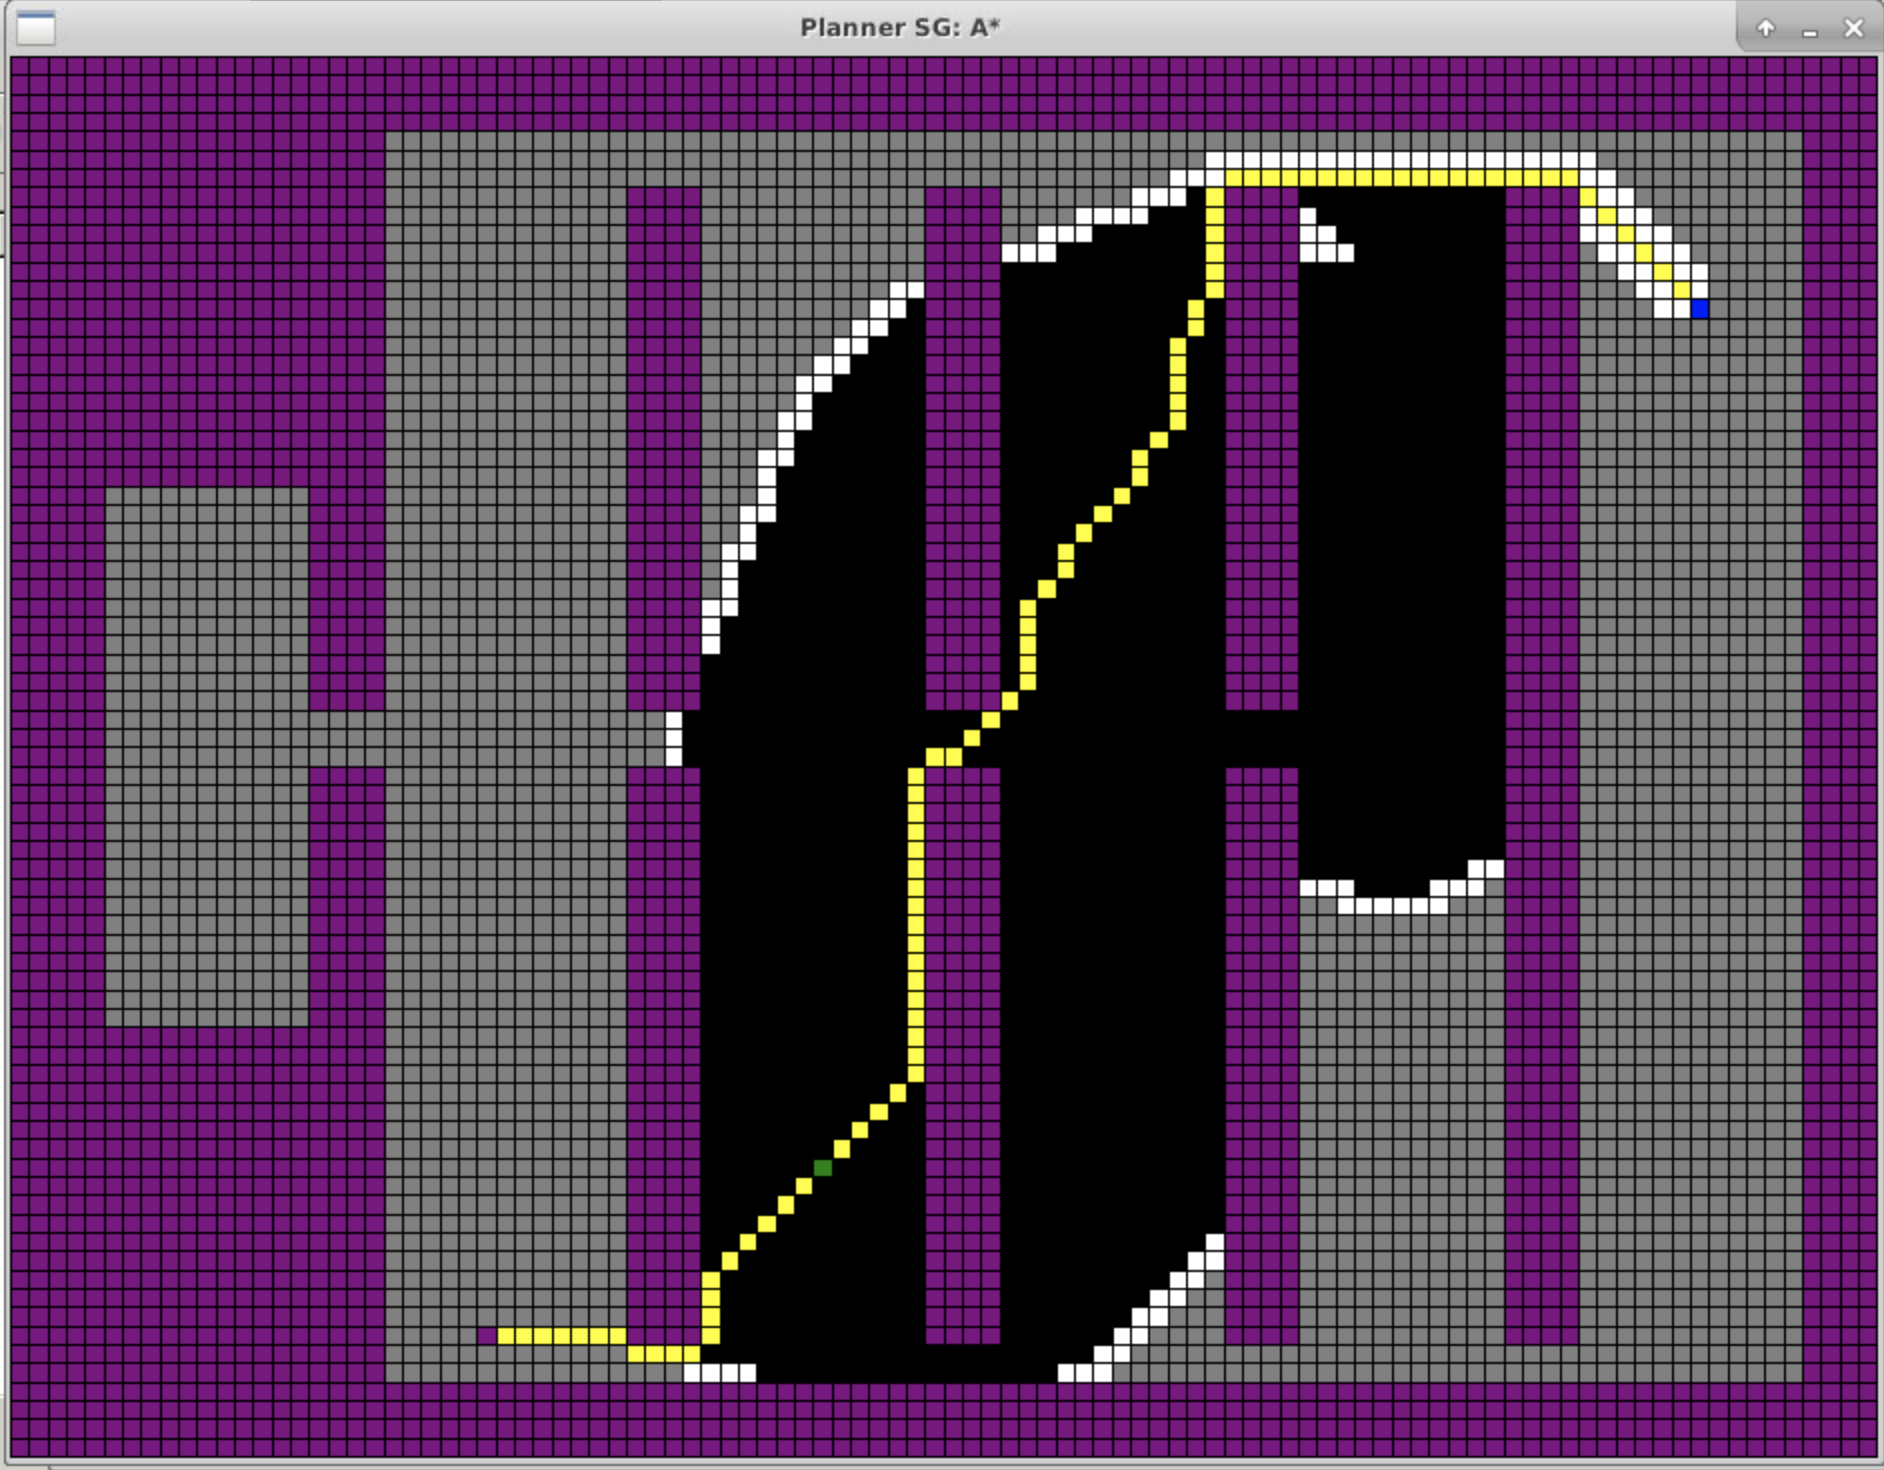
\includegraphics[width=0.32\textwidth]{graphs/part2/2-1/B.png}}
\subfigure[Via Aisle C]{
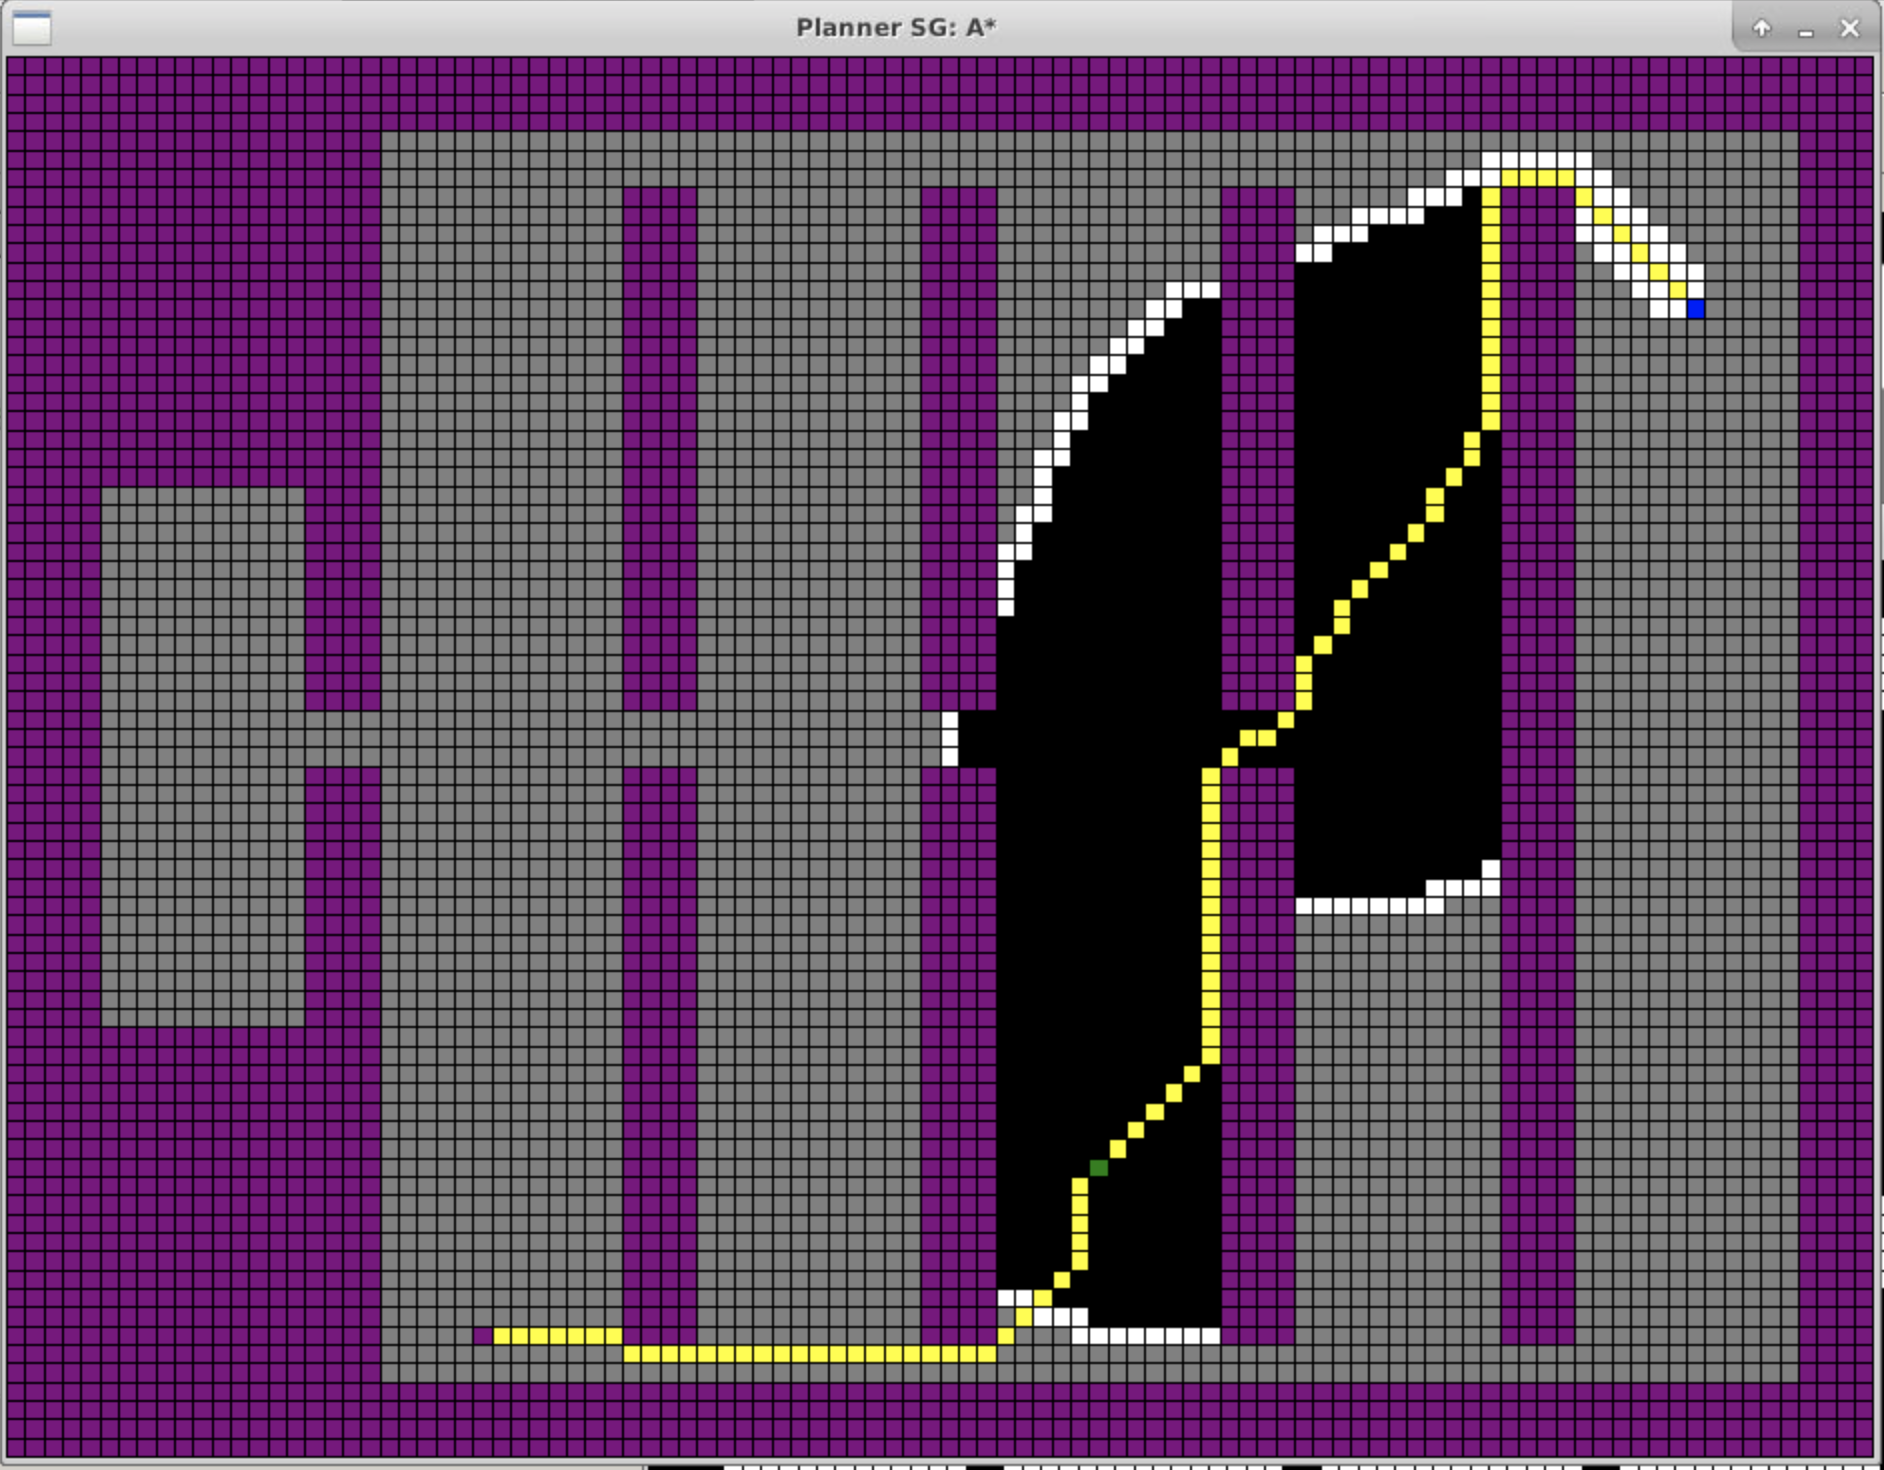
\includegraphics[width=0.32\textwidth]{graphs/part2/2-1/C.png}}
\subfigure[Via Aisle D]{
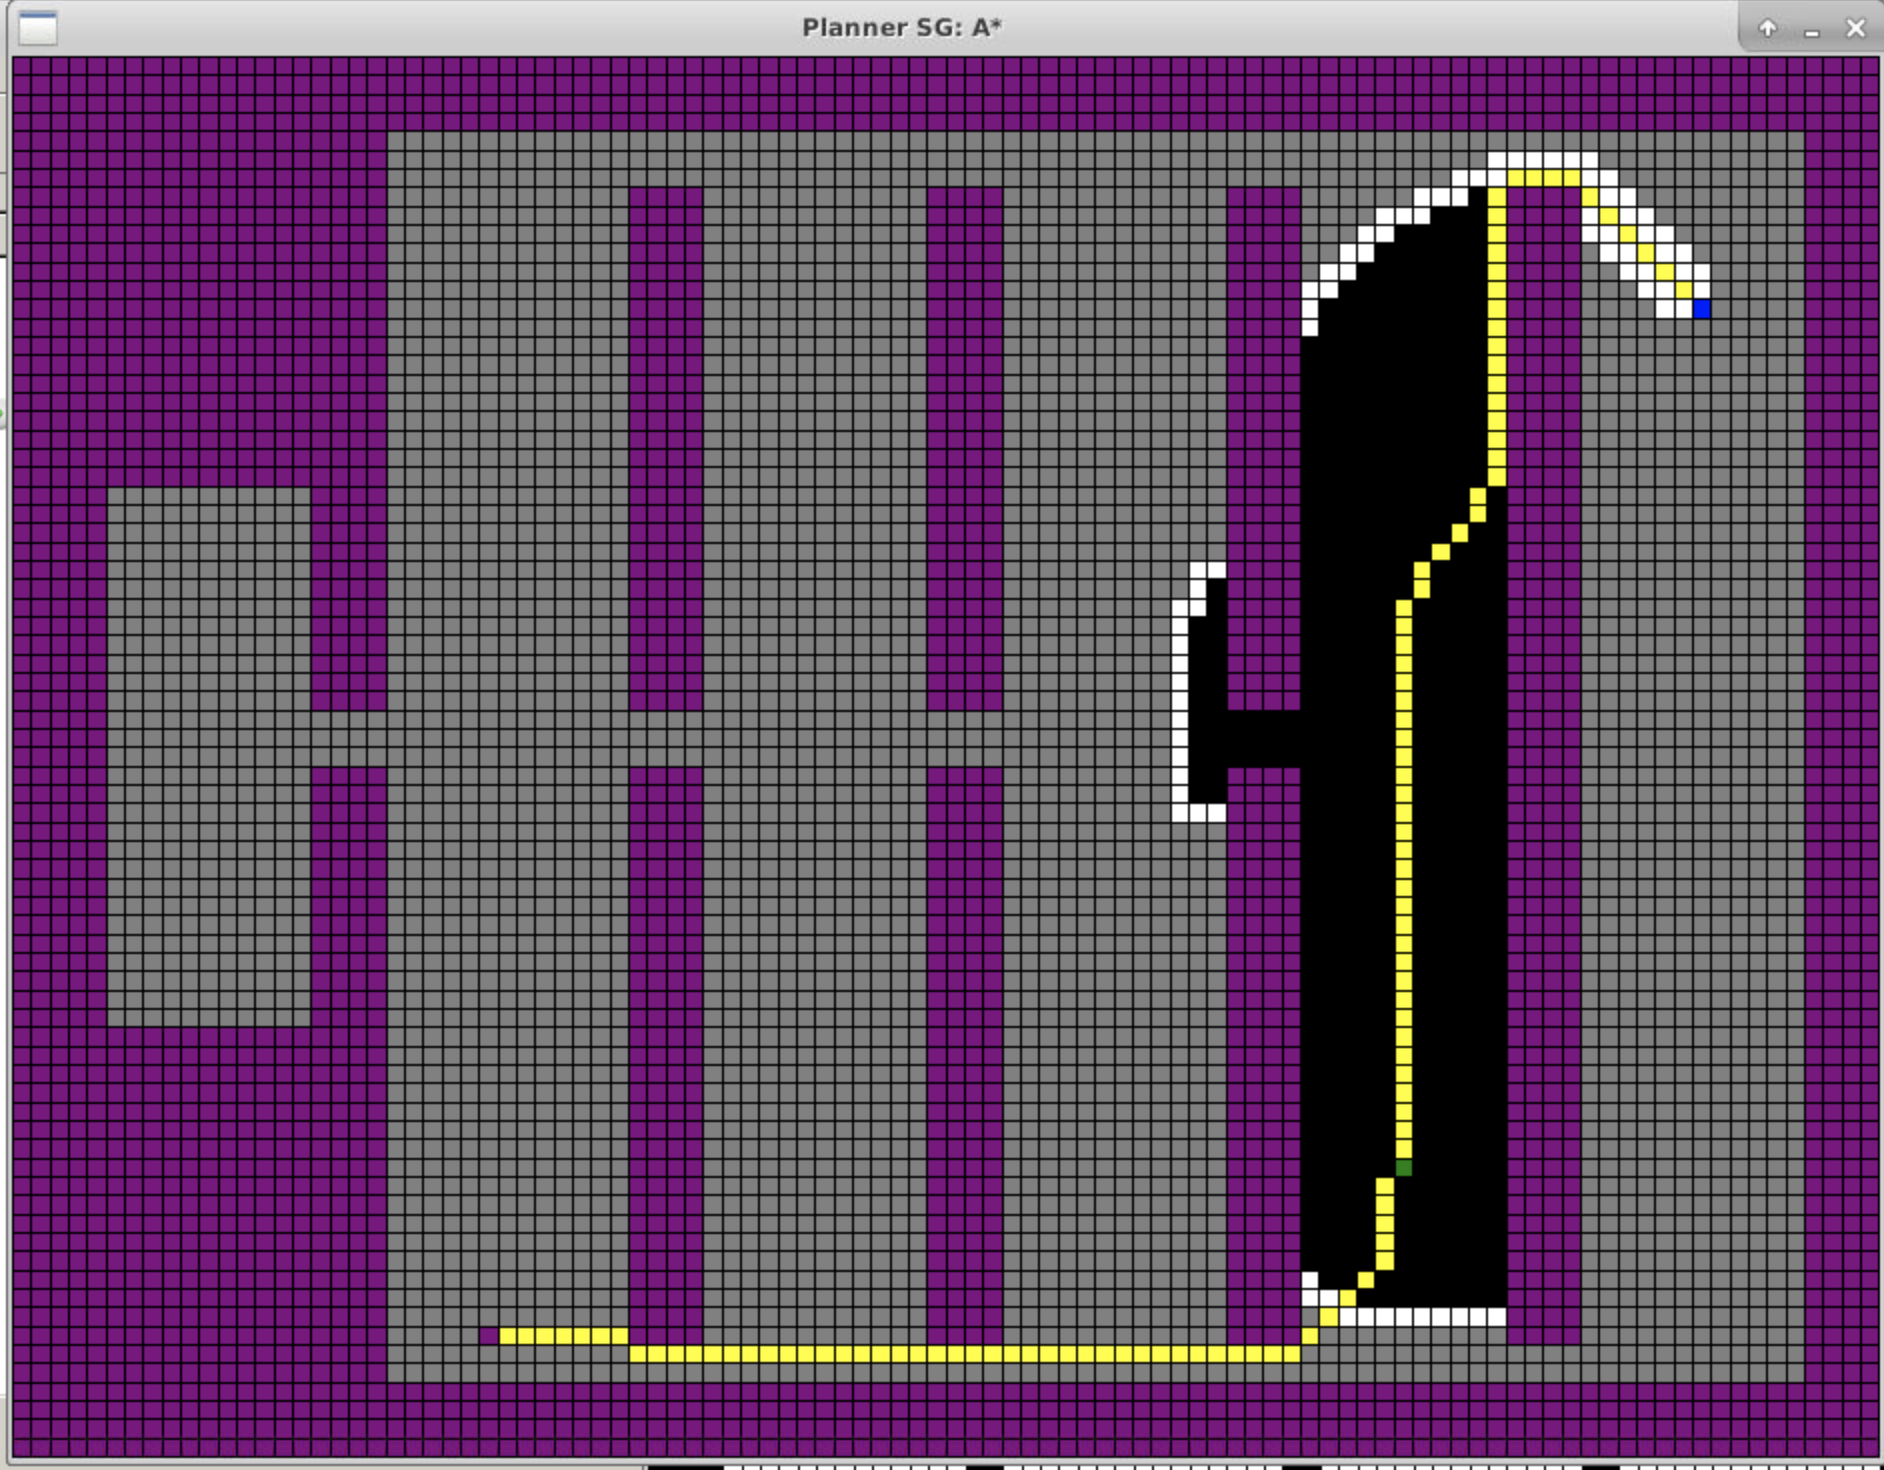
\includegraphics[width=0.35\textwidth]{graphs/part2/2-1/D.png}}
\subfigure[Via Aisle E]{
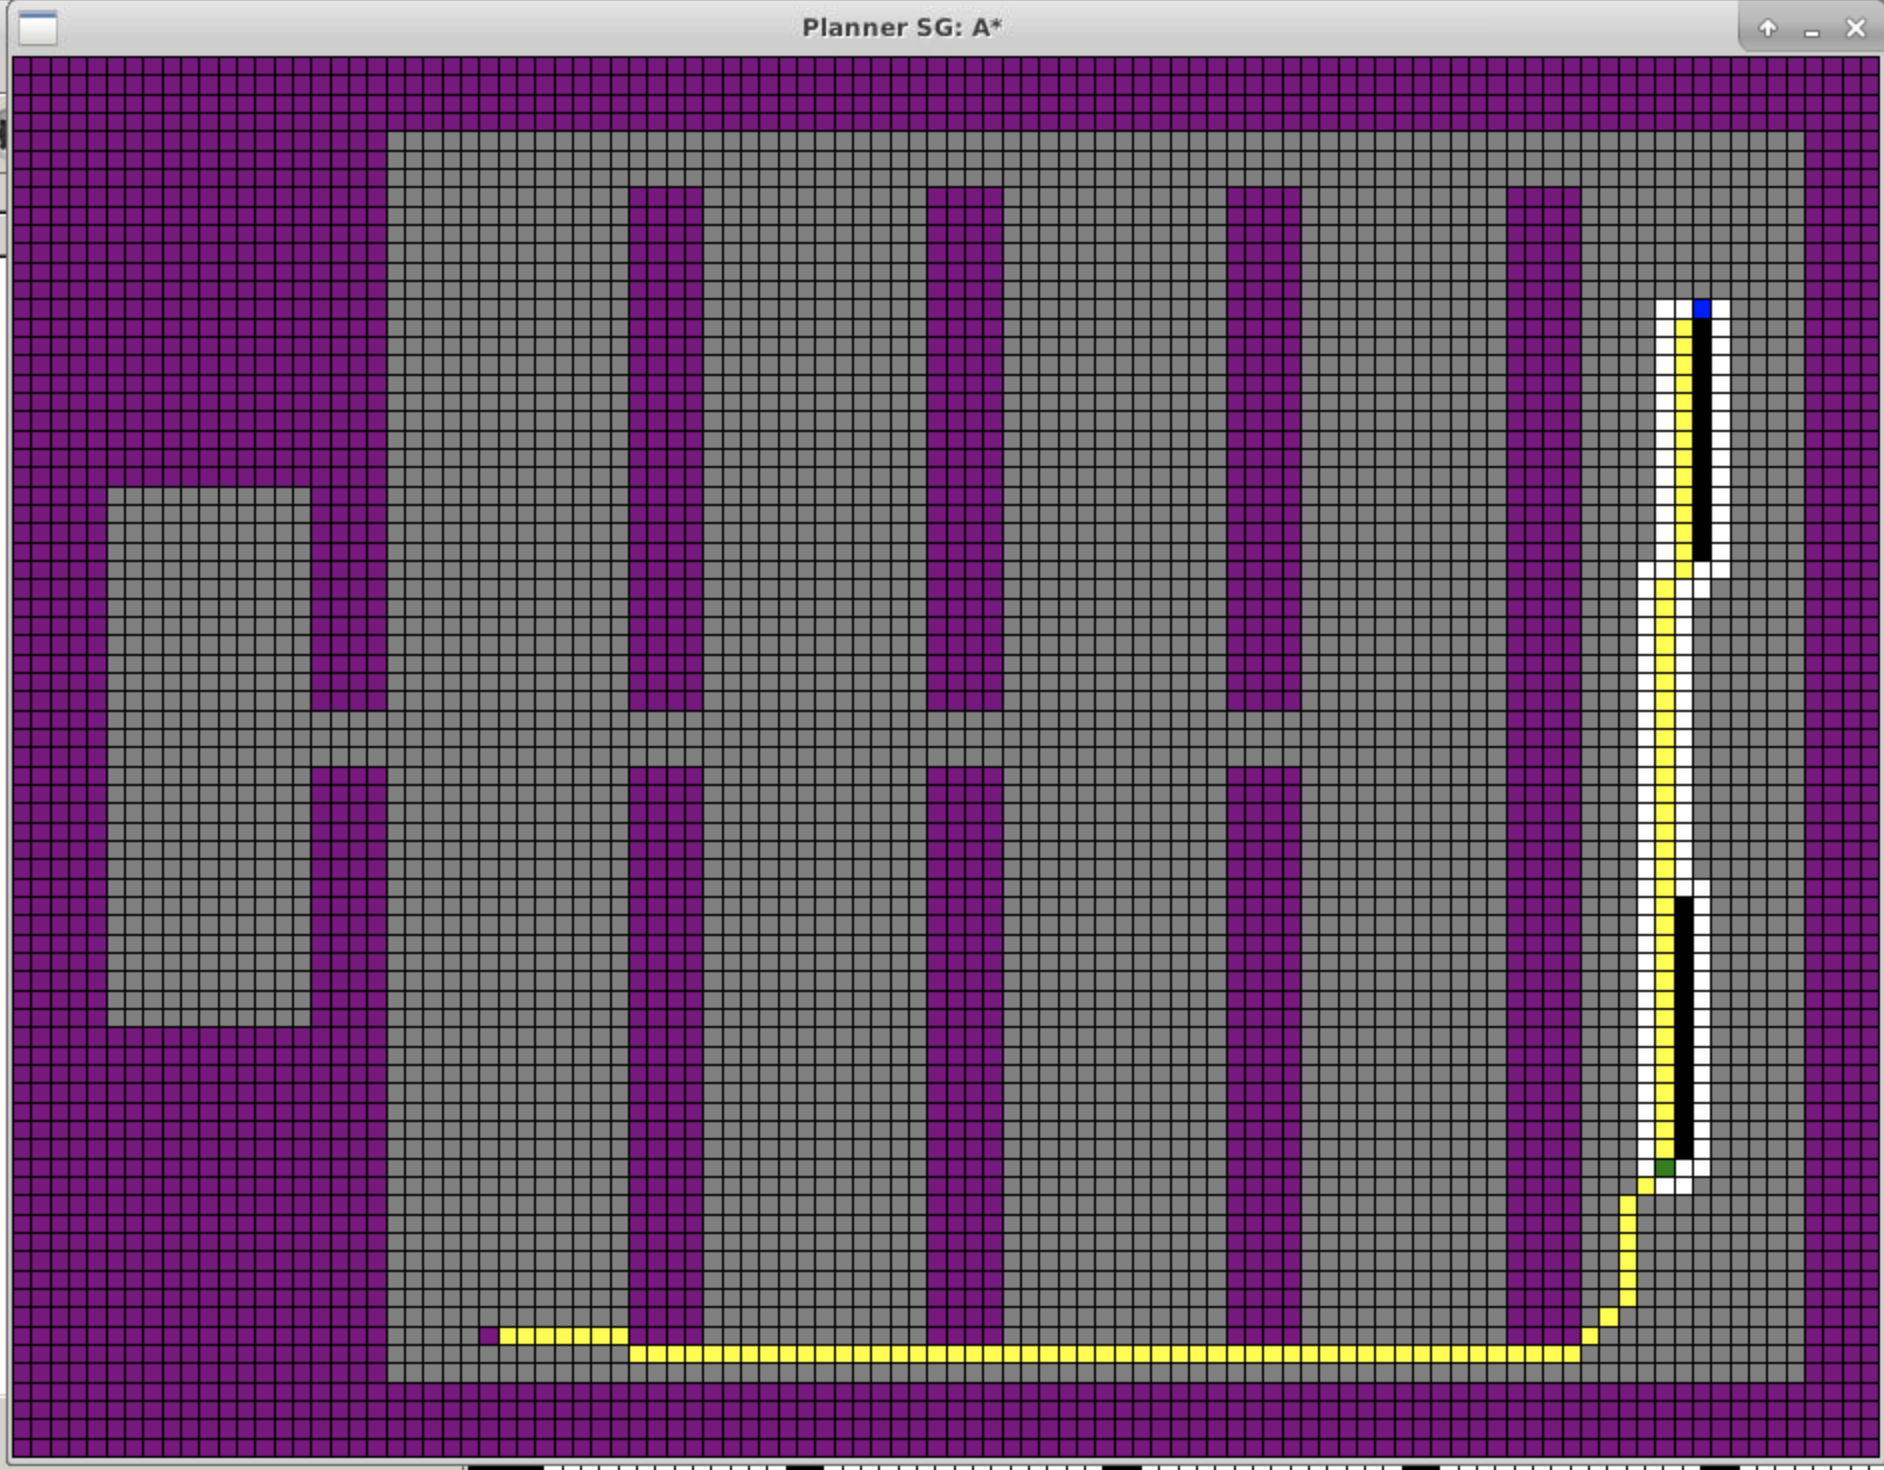
\includegraphics[width=0.35\textwidth]{graphs/part2/2-1/E.png}}
\caption{Planned Routes Down all the Different Initial Aisles}
\label{performance2.1}
\end{figure}

% ------------------
\subsection{}

% ------------------
\subsection{}

\pagebreak
% -------------------------------------------------------------------------------------------

\bibliographystyle{unsrt}  
\begin{thebibliography}{1}


 \bibitem{WFD}
 Anirudh Topiwala; Pranav Inani; Abhishek Kathpal
\newblock (2018)
\newblock Frontier Based Exploration for Autonomous Robot
\newblock {\em<https://arxiv.org/abs/1806.03581>}.

 \bibitem{2}
Brian Yamauchi
\newblock (1997)
\newblock  A Frontier-Based Approach for Autonomous Exploration
\newblock {\em<https://www.semanticscholar.org/paper/A-frontier-based-approach-for-autonomous-Yamauchi/a1875055e9c526cbdc7abb161959d76d14b58266>}.

 \bibitem{InfoTheoretic}
Callum Rhodes; Cunjia Liu; Wen-Hua Chen
\newblock (2019)
\newblock An Information Theoretic Approach to Path Planning for Frontier Exploration
\newblock {\em<https://www.researchgate.net/publication/331929185\_An\_Information\_Theoretic\_Approach\_to\_Path\_Planning\_for\_Frontier\_Exploration>}.

 \bibitem{3}
Steven M. LaValle
\newblock (2006)
\newblock Planning Algorithm
\newblock {\em<http://planning.cs.uiuc.edu>}.

 \bibitem{4}
Matan Keidar; Gal A. Kaminka
\newblock Efficient Frontier Detection for Robot Exploration
\newblock Volume: 33 issue: 2
\newblock page(s):215-236
\newblock First published online: October 22, 2013
\newblock Issue published: February 1, 2014

 \bibitem{5}
Robert M. Gray
\newblock (2013)
\newblock Entropy and Information Theory
\newblock {\em<https://ee.stanford.edu/\~gray/it.pdf>}.



\end{thebibliography}


% -----------------------------------------------------------------------------------------
\end{document}